%!TEX program = xelatex
\documentclass[11pt]{beamer}

\usepackage{amsfonts}
\usepackage{amsmath}
\usepackage{blindtext}
\usepackage{enumitem}
\usepackage{fancyvrb}
\usepackage{tikz}

%\usetheme{Recife}  % can use SaoPaulo as well
\usetheme{SaoPaulo}  % can use SaoPaulo as well

\title{MATLAB}
\subtitle{Introduction, Part II}
\author{CS101 Lecture \#22}
\date{2016-12-12}

\setcounter{showSlideNumbers}{1}

\newcommand{\correctstar}{{\Large\textcolor{red}{$\star$}}}

\begin{document}
  \setcounter{showProgressBar}{0}
  \setcounter{showSlideNumbers}{0}

%%%%%%%%%%%%%%%%%%%%%%%%%%%%%%%%%%%%%%%%%%%%%%%%%%%%%%%%%%%%%%%%%%%%%%%%%%%%%%%%
\frame{\titlepage}

%%%%%%%%%%%%%%%%%%%%%%%%%%%%%%%%%%%%%%%%%%%%%%%%%%%%%%%%%%%%%%%%%%%%%%%%%%%%%%%%
\setcounter{framenumber}{0}
\setcounter{showProgressBar}{1}
\setcounter{showSlideNumbers}{1}

%%%%%%%%%%%%%%%%%%%%%%%%%%%%%%%%%%%%%%%%%%%%%%%%%%%%%%%%%%%%%%%%%%%%%%%%%%%%%%%%
\section{Administrivia}

%%%%%%%%%%%%%%%%%%%%%%%%%%%%%%%%%%%%%%%%%%%%%%%%%%%%%%%%%%%%%%%%%%%%%%%%%%%%%%%%
\begin{frame}
  \frametitle{Administrivia}
  \Enlarge

  \begin{itemize}
  \myitem  Last Lab session this Wednesday.
  \myitem  Next Wednesday for Q\&A.
  \myitem  Homework \#9 this Thursday.
  \myitem  Grading policy for Labs/homeworks: drop the lowest grade; 25\% for Homeworks; 30\% for Final
  %\myitem  Grade check period coming up:  Dec.\ 9--14.  \pause
  \end{itemize}
\end{frame}

%%%%%%%%%%%%%%%%%%%%%%%%%%%%%%%%%%%%%%%%%%%%%%%%%%%%%%%%%%%%%%%%%%%%%%%%%%%%%%%%
\section{Warmup Questions}

%%%%%%%%%%%%%%%%%%%%%%%%%%%%%%%%%%%%%%%%%%%%%%%%%%%%%%%%%%%%%%%%%%%%%%%%%%%%%%%%
\begin{frame}[fragile]
  \frametitle{Question \#1}
  \Enlarge
$$
\left(
\begin{array}{ccc}
1 & 2 & 2 \\
2 & 1 & 2 \\
2 & 2 & 1
\end{array}
\right)
$$

How can we produce this array?

  \begin{enumerate}[label=\Alph*]
    \item  \texttt{ones(3,3) - 2*eye(3,3)}
    \item  \texttt{ones(3,3) + 2*eye(3,3)}
    \item  \texttt{2*ones(3,3) + eye(3,3)}
    \item  \texttt{2*ones(3,3) - eye(3,3)}
  \end{enumerate}
\end{frame}

%%%%%%%%%%%%%%%%%%%%%%%%%%%%%%%%%%%%%%%%%%%%%%%%%%%%%%%%%%%%%%%%%%%%%%%%%%%%%%%%
\begin{frame}[fragile]
  \frametitle{Question \#1}
  \Enlarge
$$
\left(
\begin{array}{ccc}
1 & 2 & 2 \\
2 & 1 & 2 \\
2 & 2 & 1
\end{array}
\right)
$$

How can we produce this array?

  \begin{enumerate}[label=\Alph*]
    \item  \texttt{ones(3,3) - 2*eye(3,3)}
    \item  \texttt{ones(3,3) + 2*eye(3,3)}
    \item  \texttt{2*ones(3,3) + eye(3,3)}
    \item  \texttt{2*ones(3,3) - eye(3,3)}  \correctstar
  \end{enumerate}
\end{frame}

%%%%%%%%%%%%%%%%%%%%%%%%%%%%%%%%%%%%%%%%%%%%%%%%%%%%%%%%%%%%%%%%%%%%%%%%%%%%%%%%
\begin{frame}[fragile]
  \frametitle{Question \#2}
  \Enlarge
$$
\left(
\begin{array}{cc}
1 & 2 \\
3 & 4 \\
5 & 6
\end{array}
\right)
$$

How do we access \texttt{6} in this array?

  \begin{enumerate}[label=\Alph*]
    \item  \texttt{A(2,1)}
    \item  \texttt{A(1,2)}
    \item  \texttt{A(3,2)}
    \item  \texttt{A(2,3)}
  \end{enumerate}
\end{frame}

%%%%%%%%%%%%%%%%%%%%%%%%%%%%%%%%%%%%%%%%%%%%%%%%%%%%%%%%%%%%%%%%%%%%%%%%%%%%%%%%
\begin{frame}[fragile]
  \frametitle{Question \#2}
  \Enlarge
$$
\left(
\begin{array}{cc}
1 & 2 \\
3 & 4 \\
5 & 6
\end{array}
\right)
$$

How do we access \texttt{6} in this array?

  \begin{enumerate}[label=\Alph*]
    \item  \texttt{A(2,1)}
    \item  \texttt{A(1,2)}
    \item  \texttt{A(3,2)}  \correctstar
    \item  \texttt{A(2,3)}
  \end{enumerate}
\end{frame}

%%%%%%%%%%%%%%%%%%%%%%%%%%%%%%%%%%%%%%%%%%%%%%%%%%%%%%%%%%%%%%%%%%%%%%%%%%%%%%%%
\section{MATLAB cont.d}

%%%%%%%%%%%%%%%%%%%%%%%%%%%%%%%%%%%%%%%%%%%%%%%%%%%%%%%%%%%%%%%%%%%%%%%%%%%%%%%
\begin{frame}[fragile]
  \frametitle{Basics}
  \Enlarge

  \begin{enumerate}
  \myitem  \texttt{a = [ 1 2 3 ]; \%row vector}
  \myitem  \texttt{b = [ 1 2 3 ]'; \%column vector}
  \myitem  \texttt{A = [ 1 2 3 ; 4 5 6 ]; \%matrix}
  \myitem  \texttt{B = [ a ; b ];  }
  \end{enumerate}
\end{frame}


%%%%%%%%%%%%%%%%%%%%%%%%%%%%%%%%%%%%%%%%%%%%%%%%%%%%%%%%%%%%%%%%%%%%%%%%%%%%%%%%
\begin{frame}[fragile]
  \frametitle{Indexing arrays}
  \Enlarge

  \begin{enumerate}
  \myitem  In more dimensions:
  \end{enumerate}
  \begin{semiverbatim}
A = [ 1,2,3 ; 4,5,6 ; 7,8,9 ];
B = A( 1:2,1:2 );
C = A( :,1:2 );
D = A( :,1:2:end)   \% start:interval:stop
  \end{semiverbatim}
\end{frame}

% Today will feel like a grab bag.
% Many things will be useful.  I will try to identify those that are not expected to be on an exam, however.
%TODO: check all code, add finite difference equations?

%%%%%%%%%%%%%%%%%%%%%%%%%%%%%%%%%%%%%%%%%%%%%%%%%%%%%%%%%%%%%%%%%%%%%%%%%%%%%%%%
\begin{frame}[fragile]
  \frametitle{Array Indexing}
  \Enlarge

  \begin{enumerate}
  \myitem  We can slicing an array with an array of indices.
  \end{enumerate}
  \begin{semiverbatim}
A = 0:10:100;
B = A( [ 5,9,2,2,5 ] );
  \end{semiverbatim}
\end{frame}


%%%%%%%%%%%%%%%%%%%%%%%%%%%%%%%%%%%%%%%%%%%%%%%%%%%%%%%%%%%%%%%%%%%%%%%%%%%%%%%
\begin{frame}[fragile]
	\frametitle{Matrix--Vector Operations}
	\Enlarge
	
	\begin{enumerate}
		\myitem If A is an m × n matrix (i.e., with n columns), then the product A x is defined for n × 1 column vectors x . If we let A x = b , then b is an m × 1 column vector. In other words, the number of rows in A (which can be anything) determines the number of rows in the product b. \url{http://mathinsight.org/matrix_vector_multiplication}
	\end{enumerate}
\end{frame}


%%%%%%%%%%%%%%%%%%%%%%%%%%%%%%%%%%%%%%%%%%%%%%%%%%%%%%%%%%%%%%%%%%%%%%%%%%%%%%%
\begin{frame}[fragile]
  \frametitle{Matrix--Vector Operations}
  \Enlarge

  \begin{enumerate}
  \myitem  Identity matrix does not move things
    %\begin{enumerate}
    %\mysubitem  Matrix operations are matrix--vector operations:
    %\end{enumerate}
  \end{enumerate}
  $$
\left( \begin{array}{cc}
  1 & 0 \\
  0 & 1
\end{array} \right)
\left( \begin{array}{c}
  2 \\
  3
\end{array} \right)
=
\left( \begin{array}{c}
  2 \\
  3
\end{array} \right)
  $$
  \begin{Verbatim}
[ 1 0 ; 0 1 ] * [ 2 3 ]'
  \end{Verbatim}
  \pause
  \vspace{2mm}
  $$
\left( \begin{array}{cc}
  1 & 2 \\
  1 & 1
\end{array} \right)
\left( \begin{array}{c}
  2 \\
  3
\end{array} \right)
=
\left( \begin{array}{c}
  2+3*2 \\
  2+3
\end{array} \right)
=
\left( \begin{array}{c}
  8 \\
  5
\end{array} \right)
  $$
  \begin{Verbatim}
[ 1 2 ; 1 1 ] * [ 2 3 ]'
  \end{Verbatim}
  \vspace{2mm}
  \pause
  $$
\left( \begin{array}{ccc}
  1 & 1 & 0\\
  0 & 1 & 1\\
\end{array} \right)
\left( \begin{array}{c}
  2 \\
  3 \\
  1 \\
\end{array} \right)
=
\left( \begin{array}{c}
  2+3+0\\
  0+3+1
\end{array} \right)
=
\left( \begin{array}{c}
  5 \\
  4
\end{array} \right)
  $$
  \begin{Verbatim}
[ 1 1 0; 0 1 1] * [ 2 3 1]'
  \end{Verbatim}
\end{frame}

%%%%%%%%%%%%%%%%%%%%%%%%%%%%%%%%%%%%%%%%%%%%%%%%%%%%%%%%%%%%%%%%%%%%%%%%%%%%%%%
\begin{frame}[fragile]
  \frametitle{Matrix multiplication}
  \Enlarge
  \begin{tikzpicture}[remember picture]
  \node[at=(current page.center)] {
                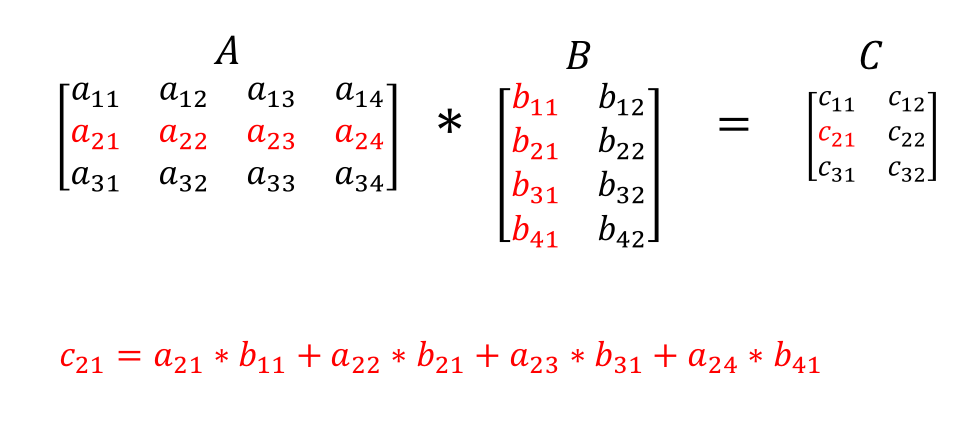
\includegraphics[height=0.4\paperheight]{./img/mult2.png}
            };
  \end{tikzpicture} \pause
  \begin{enumerate}
     \myitem  Matrix multiplications are matrix--vector operations: \pause
     	\begin{enumerate}
	\mysubitem \texttt{A*B(:,1) = C(:,1)}
	\end{enumerate}
  \end{enumerate}
\end{frame}

%%%%%%%%%%%%%%%%%%%%%%%%%%%%%%%%%%%%%%%%%%%%%%%%%%%%%%%%%%%%%%%%%%%%%%%%%%%%%%%
\begin{frame}[fragile]
  \frametitle{Elementwise operations}
  \Enlarge

  \begin{enumerate}
  \myitem  Elementwise operations are spreadsheet-like operations:
    %\begin{enumerate}
    %\mysubitem  
    %\end{enumerate}
  \end{enumerate}
  $$
\left( \begin{array}{cc}
  1 & 0 \\
  0 & 1
\end{array} \right)
\times
\left( \begin{array}{cc}
  2 & 4 \\
  3 & 5
\end{array} \right)
=
\left( \begin{array}{cc}
  2 & 0 \\
  0 & 5
\end{array} \right)
  $$
  \pause
  \begin{Verbatim}
[ 1 0 ; 0 1 ] .* [ 2 4 ; 3 5 ]
  \end{Verbatim}
\end{frame}



%%%%%%%%%%%%%%%%%%%%%%%%%%%%%%%%%%%%%%%%%%%%%%%%%%%%%%%%%%%%%%%%%%%%%%%%%%%%%%%
\begin{frame}[fragile]
  \frametitle{Multiple return values}
  \Enlarge

  \begin{enumerate}
  \myitem  Functions can return several values. 
  \end{enumerate}
  \begin{Verbatim}
function [ a,b ] = func( x )
    a = x ^ 2;
    b = x ^ 3;
end

[ q r ] = func( 3 )
  \end{Verbatim}
\end{frame}

%%%%%%%%%%%%%%%%%%%%%%%%%%%%%%%%%%%%%%%%%%%%%%%%%%%%%%%%%%%%%%%%%%%%%%%%%%%%%%%
%\begin{frame}[fragile]
%  \frametitle{Multiple returns}
%  \Enlarge

%  \begin{enumerate}
%  \myitem  But be careful---sizes cause surprises.
%  \end{enumerate}
%  %TODO
%  \begin{Verbatim}
%A = [ 'HELLO';'WORLD' ];
%A( 2,3 )
%C = [ 'HELLO';'WORLD!' ];
 % \end{Verbatim}
 % \pause
 % \begin{enumerate}
 % \myitem  How could this affect function return %values?  \pause
 % \myitem  The solution is called a \emph{cell} (but we won't cover those in 101).
 % \end{enumerate}
%\end{frame}

\iffalse
%%%%%%%%%%%%%%%%%%%%%%%%%%%%%%%%%%%%%%%%%%%%%%%%%%%%%%%%%%%%%%%%%%%%%%%%%%%%%%%
\begin{frame}[fragile]
  \frametitle{Plotting}
  \Enlarge

  \begin{enumerate}
  \myitem  \texttt{plot} works identically to \texttt{plt.plot}.  \pause
  \myitem  \texttt{figure} creates a new figure (window for plots).  \pause
  \end{enumerate}
  \begin{Verbatim}
x = 0:.1:2*pi;
y = sin( x );
figure
plot( x,y,'o' );
title( 'sin(x)' );
xlabel( 'x values' );
ylabel( 'y values' );
  \end{Verbatim}
  \pause
  \begin{enumerate}
  \myitem  MATLAB also supplies an excellent plot editor.
  \end{enumerate}
\end{frame}

%%%%%%%%%%%%%%%%%%%%%%%%%%%%%%%%%%%%%%%%%%%%%%%%%%%%%%%%%%%%%%%%%%%%%%%%%%%%%%%
\begin{frame}[fragile]
  \frametitle{Plotting}
  \Enlarge

  \begin{enumerate}
  \myitem  Here's what we have now:
    \begin{enumerate}
    \mysubitem  \texttt{function}s
    \mysubitem  array definitions, operations, slicing
    \mysubitem  plotting
    \end{enumerate}
  \pause
  \myitem  We've seen these parts---what about the rest of our ``control structures''?
  \end{enumerate}
\end{frame}
\fi



\iffalse
%%%%%%%%%%%%%%%%%%%%%%%%%%%%%%%%%%%%%%%%%%%%%%%%%%%%%%%%%%%%%%%%%%%%%%%%%%%%%%%%
\begin{frame}[fragile]
  \frametitle{\texttt{for} statement}
  \Enlarge

  \begin{itemize}
  \myitem  The \texttt{for} loop iterates over a set of possible values. \pause
  \myitem  This is \emph{not} as flexible as Python's \texttt{in} syntax---think of always having to loop over the \emph{index} rather than the item.
  \end{itemize}
\end{frame}

\fi

%%%%%%%%%%%%%%%%%%%%%%%%%%%%%%%%%%%%%%%%%%%%%%%%%%%%%%%%%%%%%%%%%%%%%%%%%%%%%%%%
\begin{frame}[fragile]
  \frametitle{\texttt{for} statement}
  \Enlarge

  \vspace{3mm}
  \begin{itemize}
  \myitem  The \texttt{for} loop iterates over a set of possible values. 
  \myitem  We create a \texttt{for} loop as follows:
    \begin{itemize}
    \mysubitem  start with \texttt{\color{red} for var = range}, where you create \texttt{var} and provide \texttt{range}
    \mysubitem  a \textbf{block} of code
    \mysubitem  closing statement \texttt{\color{red} end}
    \end{itemize}
  \pause
  \myitem  Also have \texttt{continue} and \texttt{break} available.
  \myitem  No colons
  \end{itemize}
    \begin{verbatim}
    sum = 0;
    for i = 1:100
        sum = sum + i^2;
    end
    \end{verbatim}
\end{frame}

%%%%%%%%%%%%%%%%%%%%%%%%%%%%%%%%%%%%%%%%%%%%%%%%%%%%%%%%%%%%%%%%%%%%%%%%%%%%%%%
\begin{frame}[fragile]
  \frametitle{Example: Finite difference}

  \begin{Verbatim}
%% set parameters
a = -9.8;
tmax = 0.5;     % maximum time (s)
dt = 0.01;      % time step (s)

%% data initialization
t = 0:dt:tmax;                % (s)
v = zeros(size(t));           % (m/s)
y = zeros(size(t));           % (m)
y(1) = 1;
  \end{Verbatim}
\end{frame}

%%%%%%%%%%%%%%%%%%%%%%%%%%%%%%%%%%%%%%%%%%%%%%%%%%%%%%%%%%%%%%%%%%%%%%%%%%%%%%%
\begin{frame}[fragile]
  \frametitle{Example: Finite difference}

  \begin{Verbatim}
%% loop through time steps
for i = 2:length(t)   %or numel
     v(i) = v(i-1) + a*dt;
     y(i) = y(i-1) + v(i-1)*dt;
end
  \end{Verbatim}
\end{frame}


%%%%%%%%%%%%%%%%%%%%%%%%%%%%%%%%%%%%%%%%%%%%%%%%%%%%%%%%%%%%%%%%%%%%%%%%%%%%%%%%
\begin{frame}[fragile]
  \frametitle{\texttt{if}/\texttt{else} statement}
  \Enlarge

  \begin{itemize}
  \myitem  We create an \texttt{if} statement as follows:
    \begin{itemize}
    \mysubitem  the keyword \texttt{\color{red} if}
    \mysubitem  a logical comparison  (more on this)
    \mysubitem  a \textbf{block} of code 
    \mysubitem  the keyword \texttt{\color{red} end}
    \end{itemize}
  \myitem Also have \texttt{else} and \texttt{elseif} available.
  \myitem No colons
  \end{itemize}
\end{frame}

%%%%%%%%%%%%%%%%%%%%%%%%%%%%%%%%%%%%%%%%%%%%%%%%%%%%%%%%%%%%%%%%%%%%%%%%%%%%%%%%
\begin{frame}[fragile]
  \frametitle{Example:  \texttt{absolute.m}}
  \Enlarge

  \begin{semiverbatim}
function [ y ] = absolute( x )
    y = 0;
    if x >= 0
        y = x;
    else
        y = -x;
    end
end
  \end{semiverbatim}
\end{frame}

%%%%%%%%%%%%%%%%%%%%%%%%%%%%%%%%%%%%%%%%%%%%%%%%%%%%%%%%%%%%%%%%%%%%%%%%%%%%%%%%
\begin{frame}[fragile]
  \frametitle{\texttt{while} statement}
  \Enlarge

  \begin{itemize}
  \myitem  We create an \texttt{while} statement as follows:
    \begin{itemize}
    \mysubitem  the keyword \texttt{\color{red} while}
    \mysubitem  a logical comparison
    \mysubitem  a \textbf{block} of code 
    \mysubitem  the keyword \texttt{\color{red} end}
    \end{itemize}
  \myitem Also have \texttt{continue} and \texttt{break} available.
  \myitem No colons
  \end{itemize}
\end{frame}


%%%%%%%%%%%%%%%%%%%%%%%%%%%%%%%%%%%%%%%%%%%%%%%%%%%%%%%%%%%%%%%%%%%%%%%%%%%%%%%%
\begin{frame}[fragile]
  \frametitle{The Art of MATLAB programming}
  \Enlarge

  \begin{itemize}
  \myitem  Rewrite for/while loops as built-in Matrix operations
  \begin{itemize}
  	\mysubitem  for/while loops are slow in matlab
	\mysubitem  Matlab as a high-level language is overall slower than C/C++
	\mysubitem  However, its built-in matrix/vector operations are highly optimized and very fast!
  \end{itemize}
  \myitem How?
  \end{itemize}
\end{frame}

%%%%%%%%%%%%%%%%%%%%%%%%%%%%%%%%%%%%%%%%%%%%%%%%%%%%%%%%%%%%%%%%%%%%%%%%%%%%%%%%
\begin{frame}[fragile]
  \frametitle{The Art of MATLAB programming}
  \Enlarge
  \begin{itemize}
  	\myitem Example: compute the inner product of two vectors \texttt{a} and \texttt{b}
  \end{itemize}
  \begin{semiverbatim}
  ans = 0;
  for i = 1:length(a)
      ans = ans + a(i)*b(i);
  end
  \end{semiverbatim}
  \begin{itemize}
  	\myitem What other ways to do this?
  \end{itemize}
\end{frame}

%%%%%%%%%%%%%%%%%%%%%%%%%%%%%%%%%%%%%%%%%%%%%%%%%%%%%%%%%%%%%%%%%%%%%%%%%%%%%%%%
\begin{frame}[fragile]
  \frametitle{The Art of MATLAB programming}
  \Enlarge
  \begin{itemize}
  	\myitem Exercise: find the closest number in \texttt{a} for each number in \texttt{b}
  \end{itemize}
  \begin{semiverbatim}
    a = [51  47  53   2  21  39  57  20  31   7];
    b = [56  75  13  30  35   8  30  28  90  93];
  \end{semiverbatim}
\end{frame}


\iffalse
%%%%%%%%%%%%%%%%%%%%%%%%%%%%%%%%%%%%%%%%%%%%%%%%%%%%%%%%%%%%%%%%%%%%%%%%%%%%%%%
\begin{frame}[fragile]
  \frametitle{Strings}
  \Enlarge

  \begin{enumerate}
  \myitem  Also supports strings, not as convenient as numbers (python is a better choice for handling strings) \pause
  \myitem Manages string as an array of the '\texttt{char}' type \pause
  \myitem  Enclosed with single quotes (only!).
  \end{enumerate}
  
  \begin{Verbatim}
   s = 'a brown fox';
   class(s)
   size(s)
  \end{Verbatim}
\end{frame}

\begin{frame}[fragile]
  \frametitle{String formating and print}
  \Enlarge

  \begin{enumerate}
  \myitem  Print formatted strings with \texttt{sprintf}, \texttt{fprintf}
  \begin{Verbatim}
s = sprintf( '%d %f\n', 5, sin(pi/4) ); 

%output to screen  (screen is as a file!)
fprintf('%d %f\n', 5, sin(pi/4)); 

%output to file
fp = fopen('newfile.txt', 'w')
fprintf(fp, '%d %f\n', 5, sin(pi/3));
fclose(fp)
\end{Verbatim}
\end{enumerate}
  
\end{frame}


\begin{frame}[fragile]
  \frametitle{Look for more information}
  \Enlarge

  \begin{enumerate}
    \myitem  help \texttt{func\_name}   
    	\begin{enumerate}
	\mysubitem displays help information for the function
	\end{enumerate}
    \myitem  doc \texttt{func\_name}   
    	\begin{enumerate}
	\mysubitem opens matlab's documentation
	\end{enumerate}
  \end{enumerate}

\end{frame}
%%%%%%%%%%%%%%%%%%%%%%%%%%%%%%%%%%%%%%%%%%%%%%%%%%%%%%%%%%%%%%%%%%%%%%%%%%%%%%%%

\fi


%%%%%%%%%%%%%%%%%%%%%%%%%%%%%%%%%%%%%%%%%%%%%%%%%%%%%%%%%%%%%%%%%%%%%%%%%%%%%%%%
\begin{frame}[fragile]
  \frametitle{Logical statements}
  \Enlarge

  \begin{itemize}
  \myitem  MATLAB uses the \texttt{logical} type for boolean. \pause
  \myitem  A \texttt{logical} type is 1-byte long, has values 0/1:
    \begin{itemize}
    \mysubitem  \texttt{0} means \texttt{False}
    \mysubitem  \texttt{1} means \texttt{True}
    \end{itemize}
  \pause
  \myitem  Available logical operators include:
    \begin{itemize}
    \mysubitem  \texttt{<}, \texttt{>}, \texttt{<=}, \texttt{>=}, \texttt{==},  $\~$\texttt{=}
    \mysubitem  \texttt{\&\&, \&} for AND
    \mysubitem  \texttt{||, |} for OR \pause
    \mysubitem  \texttt{\&\&, ||} are called \emph{short-circuit} logical operator \pause
    %\mysubitem  \texttt{ismember} checks equality of elements in arrays.
    \mysubitem  Can use logical operators for indexing!
    %\mysubitem  \texttt{A( A<0 )}
    \end{itemize}
  \end{itemize}
\end{frame}

%%%%%%%%%%%%%%%%%%%%%%%%%%%%%%%%%%%%%%%%%%%%%%%%%%%%%%%%%%%%%%%%%%%%%%%%%%%%%%%%
\begin{frame}[fragile]
  \frametitle{Slicing an array with logical operators}
  \Enlarge
  \begin{enumerate}
  \myitem  Slicing an array with logical operators.
  \end{enumerate}
  \begin{semiverbatim}
A = rand(10,1) - rand(10,1);
B = A( A < 0 ); %select the negative values from A 
A( A<0 ) = 0;  %set negative values in A to 0
  \end{semiverbatim}
\end{frame}




\section{File I/O}

%%%%%%%%%%%%%%%%%%%%%%%%%%%%%%%%%%%%%%%%%%%%%%%%%%%%%%%%%%%%%%%%%%%%%%%%%%%%%%%
\begin{frame}[fragile]
  \frametitle{File I/O}
  \Enlarge

  \begin{enumerate}
  \myitem  Saving data uses \texttt{'save'}:
  \begin{Verbatim}
A = [ 1 2 3 ; 4 5 6 ];
B = 5;
save( 'myvariables', 'A', 'B' );
  \end{Verbatim}
  \end{enumerate}
  \begin{enumerate}
  \myitem  Note that the \emph{string} version of the variable name is required. \pause
  \myitem  \texttt{'load'} to load the variables from saved file:
  \begin{Verbatim}
all = load('myvariables')
load( 'myvariables', 'A' );
  \end{Verbatim}
  \end{enumerate}
\end{frame}

%%%%%%%%%%%%%%%%%%%%%%%%%%%%%%%%%%%%%%%%%%%%%%%%%%%%%%%%%%%%%%%%%%%%%%%%%%%%%%%
\begin{frame}[fragile]
  \frametitle{File I/O}
  \Enlarge

  \begin{enumerate}
  \myitem  load (write) matrix data from (to) txt file: 
  \begin{Verbatim}
M = dlmread( 'rawmatdata.txt' );
dlmwrite(filename, M);
  \end{Verbatim}
  \end{enumerate}
  \pause
  \begin{enumerate}
  \myitem  ASCII-delimited \emph{numeric} data. 
  \myitem  Automatically detect delimiter in file, or user specified \pause
  \myitem  Another tool to use: \texttt{importdata} \pause
  \myitem  Old process using \texttt{fopen}, \texttt{fprintf}, \texttt{fclose} also common.
  \end{enumerate}
\end{frame}

\iffalse
%%%%%%%%%%%%%%%%%%%%%%%%%%%%%%%%%%%%%%%%%%%%%%%%%%%%%%%%%%%%%%%%%%%%%%%%%%%%%%%
\begin{frame}[fragile]
  \frametitle{File I/O}
  \Enlarge

  \begin{enumerate}
  \myitem  A more advanced (general) tool:  \texttt{importdata}
  \begin{Verbatim}
data = importdata( 'rawmatdata.txt' );
plankt = importdata('../lec12/plankton.csv');
  \end{Verbatim}
  \end{enumerate}
  \pause
  \begin{enumerate}
  %\myitem  Can be used to process CSVs.  \pause
  \myitem  Old process using \texttt{fopen}, \texttt{fprintf}, \texttt{fclose} also common.
  \end{enumerate}
\end{frame}
\fi

%%%%%%%%%%%%%%%%%%%%%%%%%%%%%%%%%%%%%%%%%%%%%%%%%%%%%%%%%%%%%%%%%%%%%%%%%%%%%%%
\begin{frame}[fragile]
  \frametitle{Images!}
  \Enlarge

  \begin{enumerate}
  \myitem  Images can also be opened as files.
  \end{enumerate}
  \begin{Verbatim}
A = imread( 'duck-color.jpg' );
imshow(A);
  \end{Verbatim}
  \pause
  \begin{enumerate}
  \myitem  A (raster) image is a grid of pixels, the size of the grid is called the \emph{resolution} (number of samples in X/Y).
  \myitem  Gray images uses a single value to denote the \emph{grayscale} for each pixel.
  \myitem  Color images usually use 3 values (R,G,B) for each pixel.  (Why?) \pause
  \myitem  Methods to display an image: \texttt{imshow}, \texttt{imagesc}, \texttt{pcolor}.
  \end{enumerate}
\end{frame}


%%%%%%%%%%%%%%%%%%%%%%%%%%%%%%%%%%%%%%%%%%%%%%%%%%%%%%%%%%%%%%%%%%%%%%%%%%%%%%%
\begin{frame}[fragile]
  \frametitle{Applications: Image processing}
  \Enlarge

  \begin{enumerate}
  \myitem  Example 1: Adjust brightness
  \myitem  Example 2: Resize an image
  \end{enumerate}

\end{frame}

%%%%%%%%%%%%%%%%%%%%%%%%%%%%%%%%%%%%%%%%%%%%%%%%%%%%%%%%%%%%%%%%%%%%%%%%%%%%%%%
\begin{frame}[fragile]
  \frametitle{Adjust brightness}
  \Enlarge

  \begin{Verbatim}
A = imread( 'duck-color.jpg' );
A = im2double(A);   %convert value to 0 - 1
B = A.^0.5;
C = A.^2;
figure; imshow(A); 
figure; imshow(B); 
figure; imshow(C);
  \end{Verbatim}

\end{frame}

%%%%%%%%%%%%%%%%%%%%%%%%%%%%%%%%%%%%%%%%%%%%%%%%%%%%%%%%%%%%%%%%%%%%%%%%%%%%%%%
\begin{frame}[fragile]
  \frametitle{Resize an image}
  \Enlarge

  
\begin{enumerate}
  \myitem  Reduce image resolution (make it smaller): \pause
\begin{Verbatim}
A = imread( 'duck-color.jpg' );
B = A(1:2:end, 1:2:end, :);
figure; imshow(A);
figure; imshow(B);
  \end{Verbatim}
\end{enumerate}

\begin{enumerate}\pause
  \myitem  How to increase the image resolution (add pixels to it)?\pause
\begin{Verbatim}
See 'img_upsample.m'
\end{Verbatim}  
\end{enumerate}

\end{frame}

\section{Plot}

%%%%%%%%%%%%%%%%%%%%%%%%%%%%%%%%%%%%%%%%%%%%%%%%%%%%%%%%%%%%%%%%%%%%%%%%%%%%%%%
\begin{frame}[fragile]
  \frametitle{Plot in Matlab}
  \Enlarge

  \begin{enumerate}
  \myitem  Open a figure: \texttt{h = figure(i)}
  \myitem  Plot in a figure: \texttt{plot}
  \myitem  Set Title: \texttt{title}
  \myitem  Set x/y label: \texttt{xlabel}, \texttt{ylabel}
  \myitem  Set range of plot: \texttt{axis([x\_min, x\_max, y\_min, y\_max])}
  \myitem  Hold on for multiple plots: \texttt{hold on}
  \myitem  Set a figure to current active window: \texttt{figure(h)}
  \end{enumerate}
  
\end{frame}


%%%%%%%%%%%%%%%%%%%%%%%%%%%%%%%%%%%%%%%%%%%%%%%%%%%%%%%%%%%%%%%%%%%%%%%%%%%%%%%
\begin{frame}[fragile]
  \frametitle{Example: plot trajectory}
  \Enlarge
  \begin{Verbatim}
  >> finite_difference
  %t,y computed for object falling trajectory
  
  h = figure;
  plot(t,y, 'b--', 'linewidth', 4);
  title('finite difference approximation');
  xlabel('time (s)');
  ylabel('height (m)');
  axis([0, 0.5, -0.5, 1]);
  \end{Verbatim}
\end{frame}

%%%%%%%%%%%%%%%%%%%%%%%%%%%%%%%%%%%%%%%%%%%%%%%%%%%%%%%%%%%%%%%%%%%%%%%%%%%%%%%
\begin{frame}[fragile]
  \frametitle{Example: plot trajectory}
  \Enlarge
  \begin{tikzpicture}[remember picture]
  \node[at=(current page.center)] {
                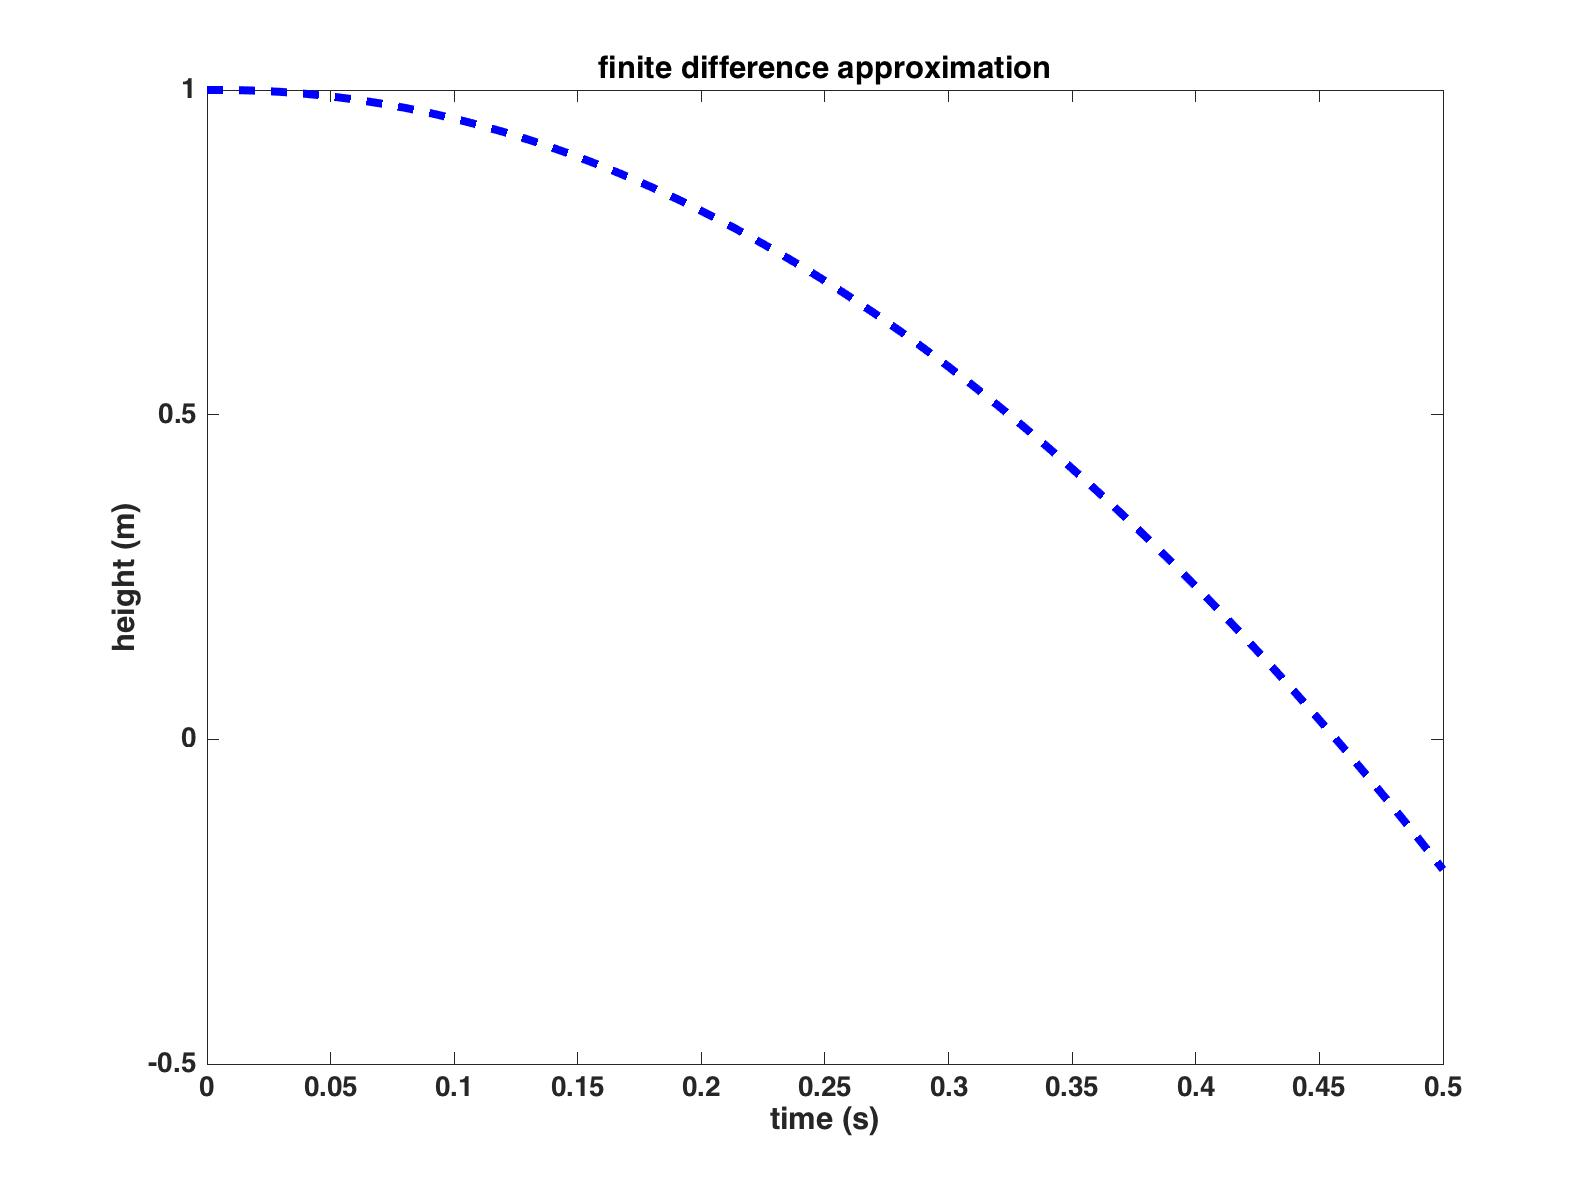
\includegraphics[height=0.75\paperheight]{./img/finite_diff.jpg}
            };
  \end{tikzpicture} 
\end{frame}

%%%%%%%%%%%%%%%%%%%%%%%%%%%%%%%%%%%%%%%%%%%%%%%%%%%%%%%%%%%%%%%%%%%%%%%%%%%%%%%
\begin{frame}[fragile]
  \frametitle{Example: plot the color mapping curves}
  \Enlarge
  \vspace{4mm}
  \begin{tikzpicture}[remember picture]
  \node[at=(current page.center)] {
                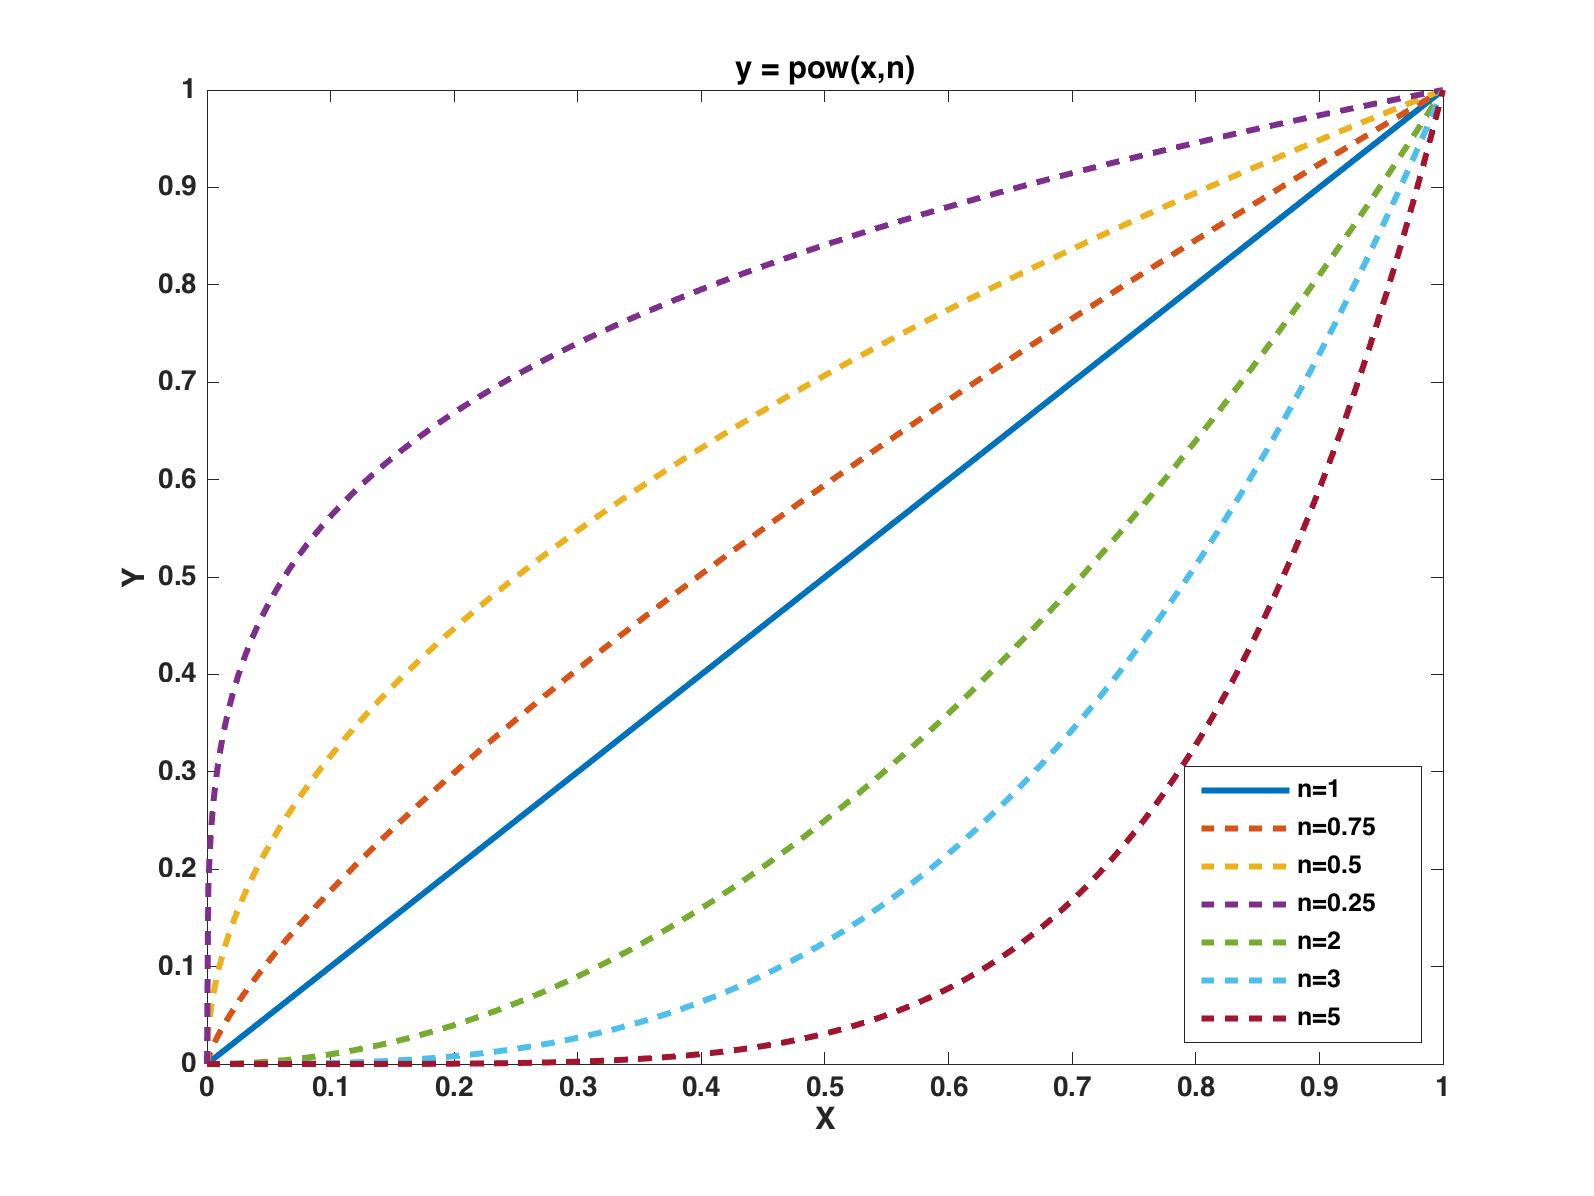
\includegraphics[height=0.75\paperheight]{./img/xpow_n.jpg}
            };
  \end{tikzpicture}
  
  See \texttt{'plot\_xpow\_n.m'}
\end{frame}


%%%%%%%%%%%%%%%%%%%%%%%%%%%%%%%%%%%%%%%%%%%%%%%%%%%%%%%%%%%%%%%%%%%%%%%%%%%%%%%
\begin{frame}[fragile]
  \frametitle{\texttt{scatter} plot}
  \Enlarge

  \begin{enumerate}
  \myitem  draw data from a Mixture of Gaussians
\begin{Verbatim}
C = 3;
center = rand(C,2)*10;
sigma = abs(randn(C,1))
  
Xs = [];
Ys = [];
for i = 1:C
   c = center(i,:);
   s = sigma(i);
  	
   Xs = [Xs; c(1) + s*randn(1000,1)];
   Ys = [Ys; c(2) + s*randn(1000,1)];
end
scatter(Xs(1:1000), Ys(1:1000), 'r');
scatter(Xs(1001:2000), Ys(1001:2000), 'g');
scatter(Xs(2001:3000), Ys(2001:3000), 'b');
\end{Verbatim} 
  \end{enumerate}

\end{frame}

%%%%%%%%%%%%%%%%%%%%%%%%%%%%%%%%%%%%%%%%%%%%%%%%%%%%%%%%%%%%%%%%%%%%%%%%%%%%%%%
\begin{frame}[fragile]
  \frametitle{Result}
  \Enlarge
  \begin{tikzpicture}[remember picture]
  \node[at=(current page.center)] {
                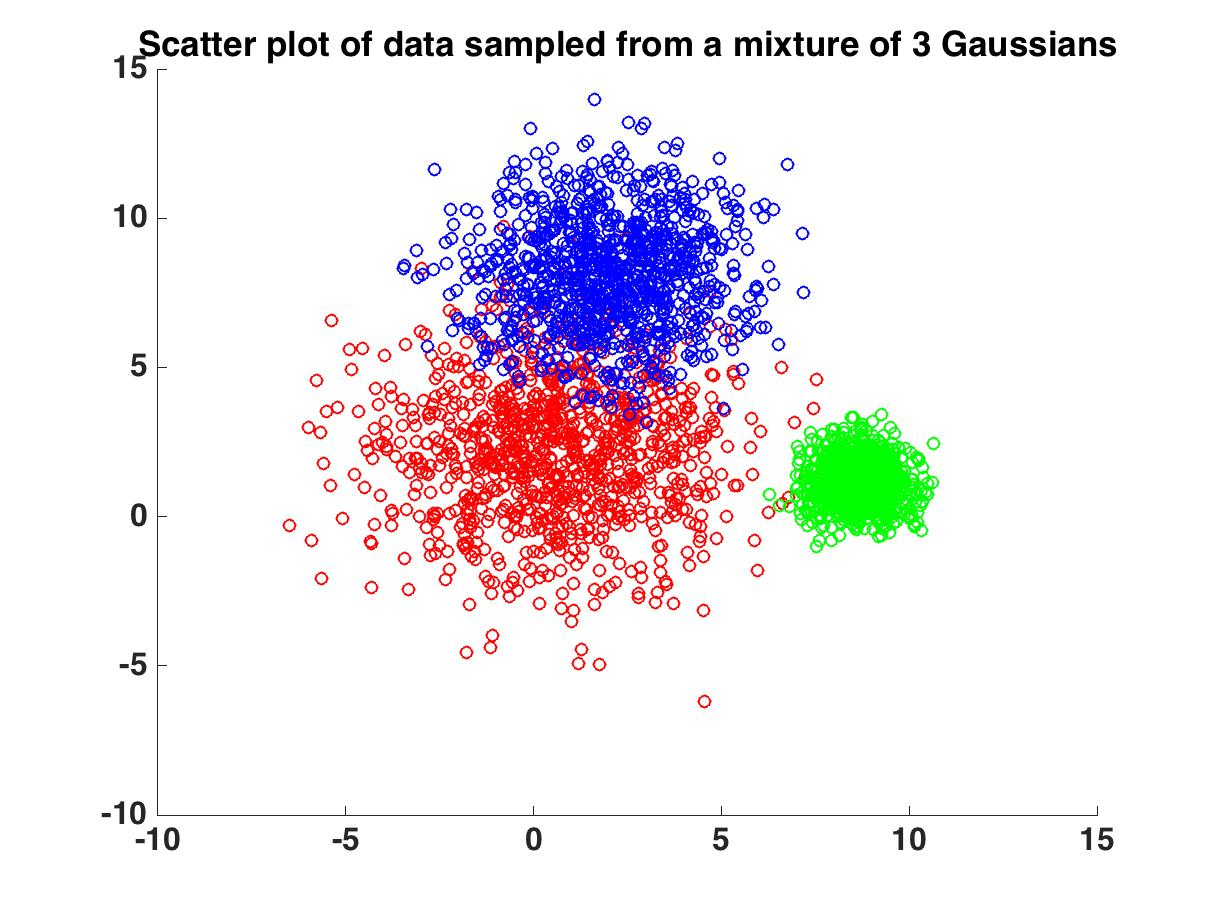
\includegraphics[height=0.75\paperheight]{./img/withlabel.jpg}
            };
  \end{tikzpicture} 
\end{frame}

%%%%%%%%%%%%%%%%%%%%%%%%%%%%%%%%%%%%%%%%%%%%%%%%%%%%%%%%%%%%%%%%%%%%%%%%%%%%%%%
\begin{frame}[fragile]
  \frametitle{Result}
  \Enlarge
  \begin{tikzpicture}[remember picture]
  \node[at=(current page.center)] {
                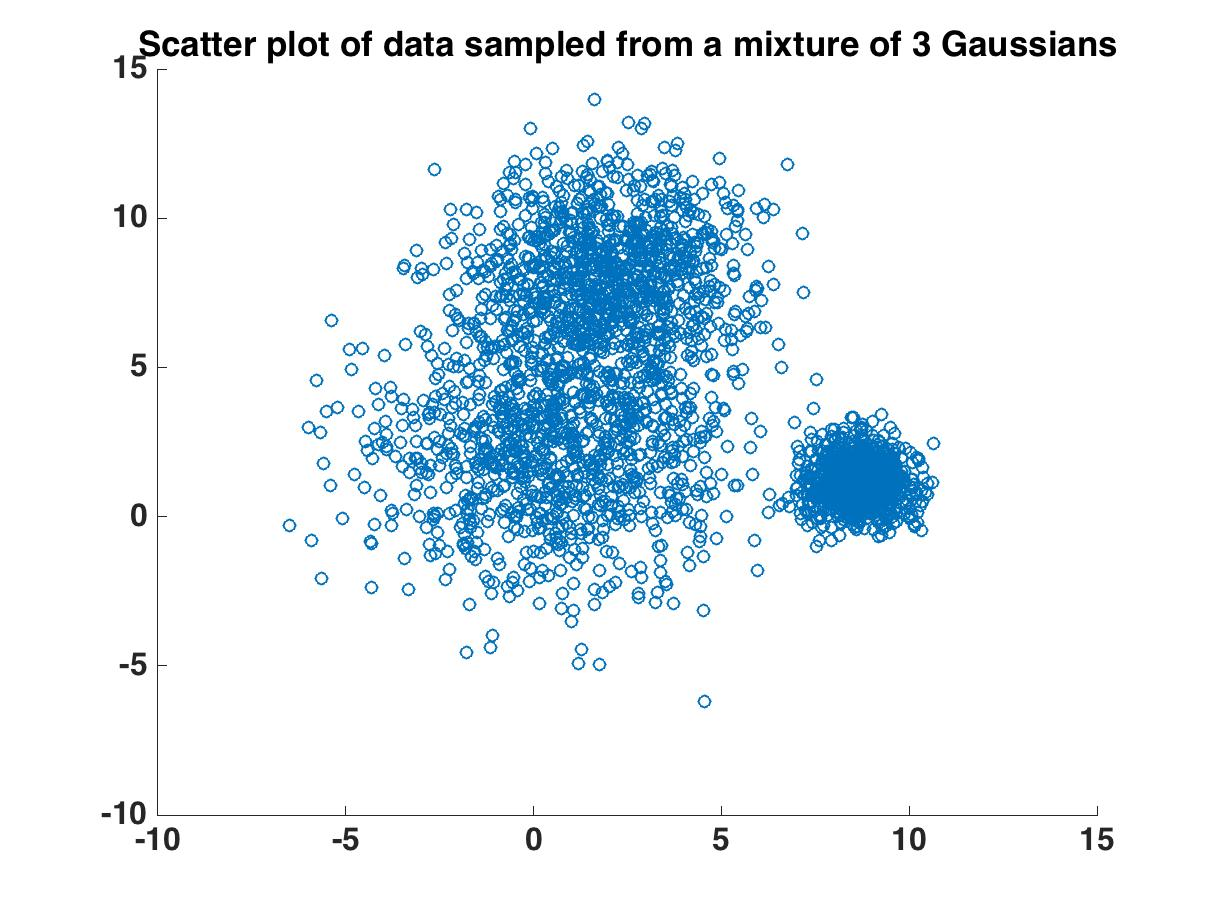
\includegraphics[height=0.75\paperheight]{./img/withoutlabel.jpg}
            };
  \end{tikzpicture} 
\end{frame}




% - PDE toolbox example?
% - find factorial using function browser

\end{document}
